\chapter{Gebruikersgevalle en -scenarios}

\section{Inleiding}
In hierdie hoofstuk word die gebruikersgevalle en -scenarios van die stelsel
beskryf. Dit sluit die verskillende gebruikersrolle in, hul interaksies met die
stelsel, en die spesifieke funksies wat beskikbaar is vir elke rol. Die
gebruikersgevalle en -scenarios bied 'n duidelike oorsig van hoe die stelsel
gebruikers se behoeftes en vereistes aanspreek, en hoe dit die algehele
gebruikerservaring verbeter.

\section{Registrasie}
\subsection{Gebruikersgeval}

\begin{figure}[htbp]
    \centering
    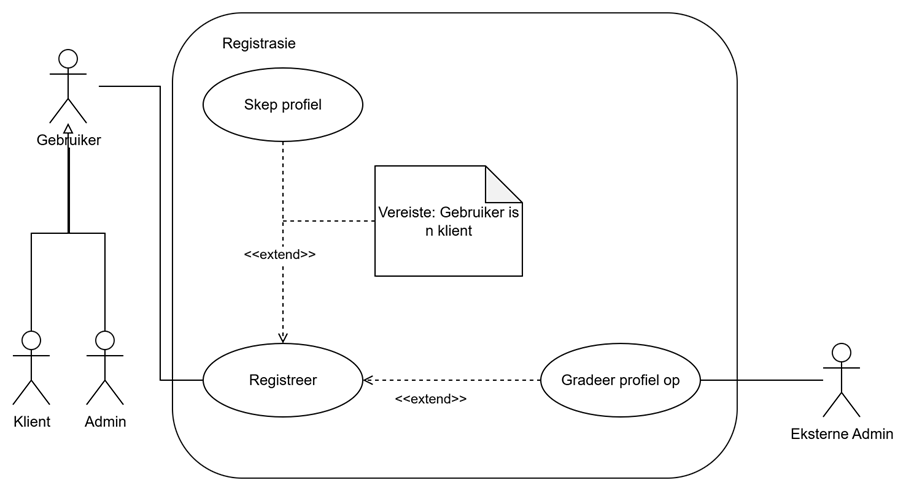
\includegraphics[width=\textwidth]{figures/usecase/registration.png}
    \caption{Gebruikersgeval vir Registrasie}
    \label{fig:registrasie_use_case}
\end{figure}

Volgens funksionele vereiste FREQ-USR-001 moet gebruikers kan registreer met hul naam en van, e-pos adres. Die registrasie proses begin op die registrasie skerm (\autoref{fig:registration_screen}). Verder volgens FREQ-USR-002 moet gebruikers wie 'n bestelling wil plaas 'n profiel skep met hul studente- of personeelnommer, kampus-ligging, koshuis indien dit van toepassing is, asook allergene indien van toepassing. Hierdie inligting word ingevul op die tweede registrasie bladsy (\autoref{fig:registration_screen_2}).

Volgens funksionele vereiste FREQ-USR-003 moet 'n administrasie profiel deur 'n ander administrasie profiel opgegradeer word vanaf 'n gewone gebruiker profiel.

\subsection{Scenario}

\textbf{Akteurs:} Gebruiker, Eksterne Administrateur\\
\textbf{Voorvereistes:} Gebruiker rekening bestaan nie\\
\textbf{Prekondisie:} Gebruiker het nie 'n rekening nie\\
\textbf{Postkondisie:} Gebruiker het 'n rekening\\
\textbf{Inset:} Gebruiker basiese inligting, Gebruiker addisionele inligting\\
\textbf{Uitset:} Sukses- of foutboodskap\\
\textbf{Skerms van Toepassing:} 
\begin{itemize}
    \item \autoref{fig:registration_screen} (Registrasie bladsy 1)
    \item \autoref{fig:registration_screen_2} (Registrasie bladsy 2)
\end{itemize}

\textbf{Hoofvloei:}
\begin{enumerate}
    \item Gebruiker navigeer na die registrasie bladsy (\autoref{fig:registration_screen})
    \item Stelsel toon registrasie vorm (\autoref{fig:registration_screen})
    \item Gebruiker vul basiese inligting in (naam, van, e-pos, wagwoord)
    \item Stelsel valideer basiese inligting
    \item Stelsel toon addisionele profiel vorm (\autoref{fig:registration_screen_2})
    \item Gebruiker vul addisionele inligting in (student/personeelnommer, kampus, koshuis, allergieë)
    \item Stelsel valideer alle inligting
    \item Stelsel skep gebruikersprofiel
    \item Gebruiker kry sukses boodskap
    \item Gebruikersgeval eindig
\end{enumerate}

\textbf{Alternatiewe vloei A1: Gebruiker wil 'n administrasie profiel maak}
\begin{enumerate}
    \item[5a.] Gebruiker sluit af.
    \item Eksterne administrateur gradeer gebruiker op
    \item Stelsel sluit die profiel vir bestellings af
    \item Gaan terug na stap 7
\end{enumerate}

\textbf{Uitsonderingsvloei E1: Ongeldige of uitgelate basiese inligting}
\begin{enumerate}
    \item[4a.] Stelsel identifiseer ongeldige of uitgelate inligting
    \item Stelsel toon foutboodskap
    \item Gaan terug na stap 3
\end{enumerate}

\textbf{Uitsonderingsvloei E2: E-pos adres bestaan reeds}
\begin{enumerate}
    \item[4b.] Stelsel identifiseer bestaande e-pos
    \item Stelsel toon "E-pos reeds geregistreer" fout
    \item Gaan terug na stap 3
\end{enumerate}

\textbf{Uitsonderingsvloei E3: Ongeldige of uitgelate addisionele inligting}
\begin{enumerate}
    \item[7a.] Stelsel identifiseer uitgelate of ongeldige addisionele inligting
    \item Stelsel toon foutboodskap
    \item Gaan terug na stap 5
\end{enumerate}

\section{Intekening}
\subsection{Gebruikersgeval}

\begin{figure}[htbp]
    \centering
    
\includegraphics[width=\textwidth]{figures/usecase/login.png}
    \caption{Gebruikersgeval vir Intekening}
    \label{fig:intekening_use_case}
\end{figure}

Volgens funksionele vereiste FREQ-USR-101 moet gebruikers inteken met 'n geldige e-pos en wagwoord kombinasie. Die intekenproses begin op die inteken skerm (\autoref{fig:login_screen}) of die administrasie portaal intekening skerm (\autoref{fig:admin_login_screen}).

Die stelsel kontroleer of die kombinasie geldig is, en skep 'n sessie vir die gebruiker.

\subsection{Scenario}

\textbf{Akteurs:} Gebruiker\\
\textbf{Voorvereistes:} Gebruiker het 'n geldige wagwoord e-pos kombinasie\\
\textbf{Prekondisie:} Gebruiker is nie ingeteken nie\\
\textbf{Postkondisie:} Gebruiker is ingeteken\\
\textbf{Inset:} Gebruiker wagwoord en e-pos kombinasie\\
\textbf{Uitset:} Sukses- of foutboodskap, sessie word geskep, navigasie na
paneelbord of hoofskerm\\
\textbf{Skerms van Toepassing:} 
\begin{itemize}
    \item \autoref{fig:login_screen} (Mobiele intekening skerm)
    \item \autoref{fig:admin_login_screen} (Administrasie portaal intekening)
\end{itemize}

\textbf{Hoofvloei:}
\begin{enumerate}
    \item Gebruiker navigeer na die inteken bladsy (\autoref{fig:login_screen})
    \item Stelsel toon intekenvorm (\autoref{fig:login_screen})
    \item Gebruiker voer e-pos adres in
    \item Gebruiker voer wagwoord in
    \item Gebruiker klik "Teken In"
    \item Stelsel valideer intekenbesonderhede
    \item Stelsel skep gebruikersessie
    \item Stelsel navigeer gebruiker na hoofbladsy of paneelbord (\autoref{fig:admin_dashboard_screen})
    \item Gebruikersgeval eindig
\end{enumerate}

\textbf{Uitsonderingsvloei E1: Uitgelate intekenbesonderhede}
\begin{enumerate}
    \item[6a.] Stelsel identifiseer uitgelate e-pos of wagwoord
    \item Stelsel toon fout boodskap
    \item Gaan terug na stap 3
\end{enumerate}

\textbf{Uitsonderingsvloei E2: Ongeldige intekenbesonderhede}
\begin{enumerate}
    \item[6b.] Stelsel identifiseer ongeldige e-pos en wagwoord kombinasie
    \item Stelsel toon "Ongeldige e-pos of wagwoord" fout
    \item Gaan terug na stap 3
\end{enumerate}

\textbf{Uitsonderingsvloei E3: Rekening is geblokkeer}
\begin{enumerate}
    \item[6c.] Stelsel identifiseer geblokkeerde rekening
    \item Stelsel toon "Rekening geblokkeer" boodskap
    \item Stelsel bied kontak besonderhede vir ondersteuning
    \item Gebruikersgeval eindig
\end{enumerate}


% Profielbestuur
\section{Profielbestuur}
\subsection{Gebruikersgeval}

\begin{figure}[htbp]
    \centering
    
\includegraphics[width=\textwidth]{figures/usecase/profile.png}
    \caption{Gebruikersgeval vir Profielbestuur}
    \label{fig:profielbestuur_use_case}
\end{figure}

Volgens FREQ-USR-201, FREQ-USR-202 en FREQ-USR-203 moet gebruikers hul profiel kan besigtig (\autoref{fig:profile_screen}) en hul koshuis en kampus ligging, allergene en wagwoord verander deur 'n profielwysigingsproses (\autoref{fig:profile_edit_screen}). Verder moet die gebruiker hul huidige rekeningbalans en transaksie geskiedenis kan sien volgens FREQ-MOB-203 en FREQ-MOB-204.

\subsection{Scenario}

\textbf{Akteurs:} Klient\\
\textbf{Voorvereistes:} Klient is ingeteken\\
\textbf{Prekondisie:} Klientprofiel is geskep\\
\textbf{Postkondisie:} Klientprofiel word gewysig\\
\textbf{Inset:} Inligting wat gewysig moet word\\
\textbf{Uitset:} Sukses- of foutboodskap\\
\textbf{Skerms van Toepassing:} 
\begin{itemize}
    \item \autoref{fig:profile_screen} (Profielbesigtig skerm)
    \item \autoref{fig:profile_edit_screen} (Profielwysiging skerm)
\end{itemize}

\textbf{Hoofvloei:}
\begin{enumerate}
    \item Gebruiker navigeer na profiel bladsy (\autoref{fig:profile_screen})
    \item Stelsel toon huidige profiel inligting (\autoref{fig:profile_screen})
    \item Stelsel toon huidige rekeningbalans
    \item Stelsel toon transaksiegeskiedenis (regs bo)
    \item Gebruiker kies om profiel te wysig (\autoref{fig:profile_edit_screen})
    \item Stelsel maak velde bewerkbaar
    \item Gebruiker wysig gewenste inligting (koshuis, kampus, allergieë, wagwoord)
    \item Gebruiker klik "Stoor Veranderinge"
    \item Stelsel valideer gewysigde inligting
    \item Stelsel werk profiel by
    \item Stelsel toon sukses boodskap
    \item Stelsel toon bygewerkte profiel inligting (\autoref{fig:profile_screen})
    \item Gebruikersgeval eindig
\end{enumerate}

\textbf{Alternatiewe vloei A1: Gebruiker kyk net profiel}
\begin{enumerate}
    \item[5a.] Gebruiker kies nie om te wysig nie
    \item Gebruikersgeval eindig
\end{enumerate}

\textbf{Alternatiewe vloei A2: Wagwoord wysiging}
\begin{enumerate}
    \item[7a.] Gebruiker kies om wagwoord te wysig
    \item Stelsel vra huidige wagwoord
    \item Stelsel vra nuwe wagwoord (twee keer)
    \item Stelsel valideer huidige wagwoord
    \item Gaan verder met stap 8
\end{enumerate}

\textbf{Uitsonderingsvloei E1: Ongeldige of uitgelate wysigings}
\begin{enumerate}
    \item[9a.] Stelsel identifiseer ongeldige of uitgelate inligting
    \item Stelsel toon foutboodskappe
    \item Gaan terug na stap 7
\end{enumerate}


% Bestellingbestuur
\section{Bestellingbestuur}
\subsection{Gebruikersgeval}

\begin{figure}[htbp]
    \centering
    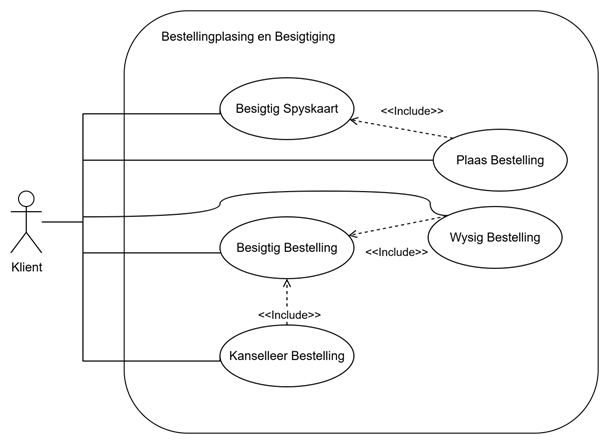
\includegraphics[width=\textwidth]{figures/usecase/orders.png}
    \caption{Gebruikersgeval vir Bestellingbestuur}
    \label{fig:bestellingbestuur_use_case}
\end{figure}

Volgens FREQ-MOB-001 moet gebruikers wat weeklikse spyskaart kan besigtig (\autoref{fig:menu_screen}), en volgens FREQ-MOB-002, FREQ-MOB-003 en FREQ-MOB-004 moet die gebruiker allergie-aanduiders, voedselwaarde en beelde van die maaltye indien beskikbaar getoon word (\autoref{fig:meal_details_screen}). Die stelsel ondersteun slegs die gebruik van 'n rekening waarvan koste gedebiteer word volgens FREQ-MOB-201. Die stelsel moet volgens FREQ-MOB-101 en FREQ-MOB-103 huidige en verlede bestellings toon (\autoref{fig:order_history_screen}).

\subsection{Scenario}

\textbf{Akteurs:} Klient\\
\textbf{Voorvereistes:} Klient is ingeteken\\
\textbf{Prekondisie:} Spyskaart is beskikbaar, gebruiker het genoegsame balans\\
\textbf{Postkondisie:} Bestelling is geplaas, gebruiker se balans word gedebiteer\\
\textbf{Inset:} Gekose Bestelling\\
\textbf{Uitset:} Sukses- of foutboodskap\\
\textbf{Skerms van Toepassing:} 
\begin{itemize}
    \item \autoref{fig:menu_screen} (Spyskaart skerm)
    \item \autoref{fig:orders_screen} (Bestelling skerm)
    \item \autoref{fig:order_success_screen} (Bestelling sukses skerm)
    \item \autoref{fig:order_error_screen} (Bestelling fout skerm)
    \item \autoref{fig:order_history_screen} (Bestelling geskiedenis skerm)
    \item \autoref{fig:meal_details_screen} (Maaltyd besonderhede skerm)
\end{itemize}


\textbf{Hoofvloei:}
\begin{enumerate}
    \item Gebruiker navigeer na spyskaart bladsy (\autoref{fig:menu_screen})
    \item Stelsel toon weeklikse spyskaart met allergie-aanduiders, voedingswaarde en beelde (\autoref{fig:menu_screen}, \autoref{fig:meal_details_screen})
    \item Gebruiker kies maaltyd(e) vir bestelling
    \item Gebruiker spesifiseer hoeveelheid
    \item Stelsel toon bestellingopsomming en totale koste
    \item Stelsel toon gebruiker se huidige rekeningbalans
    \item Gebruiker bevestig bestelling
    \item Stelsel valideer voldoende krediet
    \item Stelsel debiteer gebruiker se rekening
    \item Stelsel skep bestelling rekord
    \item Stelsel toon bestellingbevestiging (\autoref{fig:order_success_screen})
    \item Gebruikersgeval eindig
\end{enumerate}

\textbf{Alternatiewe vloei A1: Besigtig bestellings}
\begin{enumerate}
    \item[1a.] Gebruiker navigeer na "My Bestellings"
    \item Stelsel toon huidige en verlede bestellings
    \item Gebruikersgeval eindig
\end{enumerate}

\textbf{Alternatiewe vloei A2: Wysig bestaande bestelling}
\begin{enumerate}
    \item[1b.] Gebruiker kies bestaande bestelling om te wysig
    \item Stelsel kontroleer of wysiging binne tydsvenster is
    \item Stelsel toon bewerkbare bestelling
    \item Gebruikersgeval eindig
\end{enumerate}

\textbf{Alternatiewe vloei A3: Kanselleer bestelling}
\begin{enumerate}
    \item[1c.] Gebruiker kies bestaande bestelling om te kanselleer
    \item Stelsel kontroleer of kansellasie binne tydsvenster is
    \item Stelsel vra bevestiging vir kansellasie
    \item Gebruiker bevestig kansellasie
    \item Stelsel kanselleer bestelling en krediteer rekening
    \item Stelsel toon kansellasiebevestiging
\end{enumerate}

\textbf{Uitsonderingsvloei E1: Onvoldoende krediet}
\begin{enumerate}
    \item[8a.] Stelsel identifiseer onvoldoende krediet
    \item Stelsel toon "Onvoldoende krediet" fout
    \item Stelsel toon huidige balans en benodigde bedrag
    \item Stelsel bied opsie om admin te kontak
    \item Gebruikersgeval eindig
\end{enumerate}

\textbf{Uitsonderingsvloei E2: Wysiging/kansellasie buite tydsvenster}
\begin{enumerate}
    \item[1d.] Stelsel identifiseer dat tydsvenster verby is
    \item Stelsel toon "Te laat vir wysigings" boodskap
    \item Gebruikersgeval eindig
\end{enumerate}


% Terugvoer
\section{Terugvoer}
\subsection{Gebruikersgeval}

\begin{figure}[htbp]
    \centering
    
\includegraphics[width=\textwidth]{figures/usecase/feedback.png}
    \caption{Gebruikersgeval vir Terugvoer}
    \label{fig:terugvoer_use_case}
\end{figure}

Volgens FREQ-MOB-301, FREQ-MOB-302 en FREQ-MOB-303 het gebruikers die keuse om terugvoer te verskaf op 'n 5-punt skaal (\autoref{fig:feedback_screen}), en kommentaar te lewer oor die maaltyd slegs beskikbaar vir admin personeel. Na suksesvolle indiening word die terugvoer sukses skerm getoon (\autoref{fig:feedback_success_screen}).

\subsection{Scenario}

\textbf{Akteurs:} Klient\\
\textbf{Voorvereistes:} Klient is ingeteken\\
\textbf{Prekondisie:} Minstens een geskiedkundige bestelling\\
\textbf{Postkondisie:} Terugvoer word gelewer\\
\textbf{Inset:} 5-punt skaal waarde, kommentaar\\
\textbf{Uitset:} Sukses- of foutboodskap\\
\textbf{Skerms van Toepassing:} 
\begin{itemize}
    \item \autoref{fig:feedback_screen} (Terugvoer skerm)
    \item \autoref{fig:feedback_success_screen} (Terugvoer sukses skerm)
\end{itemize}


\textbf{Hoofvloei:}
\begin{enumerate}
    \item Gebruiker navigeer na terugvoer bladsy of kies bestelling vir terugvoer (\autoref{fig:feedback_screen})
    \item Stelsel toon lys van voltooide bestellings beskikbaar vir terugvoer
    \item Gebruiker kies spesifieke maaltyd/bestelling
    \item Stelsel toon terugvoervorm (\autoref{fig:feedback_screen})
    \item Gebruiker gee gradering op 5-punt skaal
    \item Gebruiker voer opsionele kommentaar in
    \item Gebruiker dien terugvoer in
    \item Stelsel stoor terugvoer 
    \item Stelsel toon bevestiging boodskap (\autoref{fig:feedback_success_screen})
    \item Gebruikersgeval eindig
\end{enumerate}

\textbf{Uitsonderingsvloei E1: Geen voltooide bestellings}
\begin{enumerate}
    \item[2a.] Stelsel identifiseer geen voltooide bestellings
    \item Stelsel toon "Geen bestellings beskikbaar vir terugvoer"
    \item Gebruikersgeval eindig
\end{enumerate}


% Spyskaartbestuur
\section{Spyskaartbestuur}
\subsection{Gebruikersgeval}

\begin{figure}[htbp]
    \centering
    
\includegraphics[width=\textwidth]{figures/usecase/menu.png}
    \caption{Gebruikersgeval vir Spyskaartbestuur}
    \label{fig:spyskaartbestuur_use_case}
\end{figure}

Volgens FREQ-WEB-001, FREQ-WEB-002 en FREQ-WEB-003 moet die administrasie portaal die skep en wysiging van die weeklikse ete van die dag spyskaart insluit (\autoref{fig:menu_management_screen}). Die mobiele spyskaart kan besigtig word op die spyskaart skerm (\autoref{fig:menu_screen}).

\subsection{Scenario}

\textbf{Akteurs:} Admin\\
\textbf{Voorvereistes:} Admin is ingeteken, Admin het die korrekte regte\\
\textbf{Prekondisie:} Spyskaart bestaan nie of gekose spyskaart bestaan\\
\textbf{Postkondisie:} Spyskaart geskep of gewysig\\
\textbf{Inset:} Spyskaart informasie\\
\textbf{Uitset:} Sukses- of foutboodskap\\
\textbf{Skerms van Toepassing:} 
\begin{itemize}
    \item \autoref{fig:menu_management_screen} (Spyskaartbestuur skerm - admin)
    \item \autoref{fig:menu_screen} (Spyskaart skerm - mobiel)
\end{itemize}


\textbf{Hoofvloei:}
\begin{enumerate}
    \item Administrasie gebruiker teken in na web portaal
    \item Stelsel toon admin dashboard
    \item Admin navigeer na spyskaart bestuur (\autoref{fig:menu_management_screen})
    \item Stelsel toon huidige weeklikse spyskaart (\autoref{fig:menu_management_screen})
    \item Admin kies om nuwe spyskaart te skep
    \item Stelsel toon spyskaartwysigingsvorm (\autoref{fig:menu_management_screen})
    \item Admin voer/wysig maaltydbesonderhede (naam, beskrywing, prys)
    \item Admin voeg allergie-inligting by
    \item Admin voeg voedingswaarde-inligting by
    \item Admin laai maaltyd beelde op (indien beskikbaar)
    \item Admin stoor veranderinge
    \item Stelsel valideer alle inligting
    \item Stelsel werk spyskaart by
    \item Stelsel toon sukses bevestiging
    \item Gebruikersgeval eindig
\end{enumerate}

\textbf{Alternatiewe vloei A1: Wysig bestaande maaltyd}
\begin{enumerate}
    \item[5a.] Admin kies om bestaande maaltyd te wysig
    \item Stelsel gaan haal bestaande maaltyd besonderhede
    \item Gaan na stap 6
\end{enumerate}

\textbf{Alternatiewe vloei A2: Verwyder maaltyd}
\begin{enumerate}
    \item[5b.] Admin kies om maaltyd te verwyder
    \item Stelsel vra bevestiging
    \item Admin bevestig verwydering
    \item Stelsel verwyder maaltyd van spyskaart
    \item Gebruikersgeval eindig
\end{enumerate}

\textbf{Uitsonderingsvloei E1: Ongeldige maaltyd inligting}
\begin{enumerate}
    \item[12a.] Stelsel identifiseer ongeldige inligting
    \item Stelsel toon foutboodskappe
    \item Gaan terug na stap 7
\end{enumerate}


% Verslaggewing
\section{Verslaggewing}
\subsection{Gebruikersgeval}

\begin{figure}[htbp]
    \centering
    
\includegraphics[width=\textwidth]{figures/usecase/report.png}
    \caption{Gebruikersgeval vir Verslaggewing}
    \label{fig:verslaggewing_use_case}
\end{figure}

Volgens FREQ-WEB-102 en FREQ-WEB-103 moet finansiële verslae oor die balans van gebruikers op die stelsel, asook statistiek soos hoeveel deur gebruikers bestee word op die platform gegenereer kan word. Hierdie verslae word besigtig op die verslaggewing skerm (\autoref{fig:report_screen}). Verder volg FREQ-WEB-201 en FREQ-WEB-202 dat versale oor die huidige, verlede en gekansellerde bestellings gegenereer kan word, asook 'n verslag oor aantal etes wat voorberei moet word.

\subsection{Scenario}

\textbf{Akteurs:} Admin\\
\textbf{Voorvereistes:} Admin is ingeteken, Admin het die korrekte regte\\
\textbf{Prekondisie:} Inligting is beskikbaar vir 'n gegewe tydsreeks\\
\textbf{Postkondisie:} Verslag is beskikbaar\\
\textbf{Inset:} Tipe verslag, Verslag parameters, Datumreeks\\
\textbf{Uitset:} Sukses- of foutboodskap\\
\textbf{Skerms van Toepassing:} 
\begin{itemize}
    \item \autoref{fig:report_screen} (Verslaggewing skerm)
\end{itemize}

\textbf{Hoofvloei:}
\begin{enumerate}
    \item Administrasie gebruiker navigeer na verslag afdeling (\autoref{fig:report_screen})
    \item Stelsel toon beskikbare verslag opsies (\autoref{fig:report_screen})
    \item Admin kies verslag tipe 
    \item Stelsel toon verslag parameters vorm
    \item Admin spesifiseer datumreeks
    \item Admin spesifiseer addisionele filters (indien van toepassing)
    \item Admin klik "Genereer Verslag"
    \item Stelsel versamel relevante data
    \item Stelsel genereer verslag
    \item Stelsel toon verslag aan admin (\autoref{fig:report_screen})
    \item Admin kan verslag aflaai of druk
    \item Gebruikersgeval eindig
\end{enumerate}

\textbf{Uitsonderingsvloei E1: Geen data vir gekose periode}
\begin{enumerate}
    \item[8a.] Stelsel vind geen data vir parameters
    \item Stelsel toon "Geen data beskikbaar"
    \item Stelsel bied opsie om parameters te wysig
    \item Gaan terug na stap 5
\end{enumerate}



% Finansiële Administrasie
\section{Finansiële Administrasie}
\subsection{Gebruikersgeval}

\begin{figure}[htbp]
    \centering
    
\includegraphics[width=\textwidth]{figures/usecase/finance.png}
    \caption{Gebruikersgeval vir Finansiële Administrasie}
    \label{fig:finansiele_admin_use_case}
\end{figure}

Volgens FREQ-WEB-101 moet administrasie gebruikers krediet inlees vir gebruikersrekeninge. Die finansiële administrasie proses word uitgevoer op die finansiële administrasie skerm (\autoref{fig:finance_management_screen}).

\subsection{Scenario}

\textbf{Akteurs:} Admin\\
\textbf{Voorvereistes:} Admin is ingeteken, Admin het die korrekte regte\\
\textbf{Prekondisie:} Minstens een Klient bestaan\\
\textbf{Postkondisie:} Gebruiker se rekening aangepas\\
\textbf{Inset:} Gebruikers inligting, aantal Krediet/Debiet\\
\textbf{Uitset:} Sukses- of foutboodskap\\
\textbf{Skerms van Toepassing:} 
\begin{itemize}
    \item \autoref{fig:finance_management_screen} (Finansiële Administrasie skerm)
\end{itemize}

\textbf{Hoofvloei:}
\begin{enumerate}
    \item Administrasie gebruiker navigeer na krediet bestuur (\autoref{fig:finance_management_screen})
    \item Stelsel toon gebruiker soek funksie
    \item Admin soek vir gebruiker (naam, e-pos, of studentnommer)
    \item Stelsel toon soekresultate
    \item Admin kies korrekte gebruiker
    \item Stelsel toon gebruiker se huidige balans en transaksie geskiedenis (\autoref{fig:finance_management_screen})
    \item Admin voer krediet bedrag in om by te voeg
    \item Admin voeg verwysing by
    \item Admin bevestig krediet toevoeging
    \item Stelsel valideer bedrag
    \item Stelsel werk gebruiker se balans by
    \item Stelsel skep transaksierekord
    \item Stelsel toon sukses bevestiging met nuwe balans (\autoref{fig:finance_management_screen})
    \item Gebruikersgeval eindig
\end{enumerate}

\textbf{Alternatiewe vloei A1: Bulk krediet laai}
\begin{enumerate}
    \item[3a.] Admin kies bulk krediet opsie
    \item Stelsel bied CSV oplaai
    \item Admin laai CSV lêer op met gebruiker besonderhede en bedrae
    \item Stelsel verifieer lêer formaat
    \item Stelsel verifieer studente/personeel nommers.
    \item Stelsel prosesseer alle krediterings
    \item Stelsel toon opsomming van sukses/onsuksesvolle transaksies
\end{enumerate}

\textbf{Alternatiewe vloei A2: Debiteer rekening}
\begin{enumerate}
    \item[7a.] Admin voer negatiewe bedrag in (debitering)
    \item Stelsel vra bevestiging vir debitering
    \item Gaan na stap 9
\end{enumerate}

\textbf{Uitsonderingsvloei E1: Gebruiker nie gevind}
\begin{enumerate}
    \item[4a.] Stelsel vind geen passende gebruikers
    \item Stelsel toon "Geen gebruikers gevind nie"
    \item Gaan terug na stap 3
\end{enumerate}

\textbf{Uitsonderingsvloei E2: Gebruiker nie gevind in bulk krediet transaksie}
\begin{enumerate}
    \item[4b.] Stelsel vind nie 'n gebruiker in 'n rekord nie.
    \item Stelsel toon die rekords wat nie pas nie
    \item Gaan terug na stap 3
\end{enumerate}


% Gebruiker en Toegangsbeheer
\section{Gebruiker en Toegangsbeheer}
\subsection{Gebruikersgeval}

\begin{figure}[htbp]
    \centering
    
\includegraphics[width=\textwidth]{figures/usecase/management.png}
    \caption{Gebruikersgeval vir Gebruiker en Toegangsbeheer}
    \label{fig:gebruiker_toegangsbeheer_use_case}
\end{figure}

Volgens FREQ-WEB-301, FREQ-WEB-302 en FREQ-WEB-303 moet administrasie gebruikers kan toegangsregte en toegangsgeskiedenis van gebruikers sien asook rol en toegangsregte wysig. Hierdie funksies word uitgevoer op die gebruikerswysiging skerm (\autoref{fig:user_edit_screen}).

Verder moet die stelsel funksionaliteit bied om kennisgewings aan gebruikers te stuur (FREQ-WEB-304).

\subsection{Scenario}

\textbf{Akteurs:} Admin\\
\textbf{Voorvereistes:} Admin is ingeteken, Admin het die korrekte regte\\
\textbf{Prekondisie:} Minstens een gebruiker anders as admin bestaan\\
\textbf{Postkondisie:} Gebruiker rol en toegang verander\\
\textbf{Inset:} Gebruiker, gebruiker rolle, blokasie (ja, ne)\\
\textbf{Uitset:} Sukses- of foutboodskap\\
\textbf{Skerms van Toepassing:} 
\begin{itemize}
    \item \autoref{fig:user_edit_screen} (Gebruikerswysiging skerm)
\end{itemize}


\textbf{Hoofvloei:}
\begin{enumerate}
    \item Administrasie gebruiker navigeer na gebruiker bestuur (\autoref{fig:user_edit_screen})
    \item Stelsel toon gebruiker bestuur dashboard (\autoref{fig:user_edit_screen})
    \item Admin soek vir spesifieke gebruiker of blaai deur gebruiker lys
    \item Stelsel toon gebruiker lys met basiese inligting
    \item Admin kies gebruiker om te bestuur (\autoref{fig:user_edit_screen})
    \item Stelsel toon gebruiker besonderhede, rol, en toegangsgeskiedenis (\autoref{fig:user_edit_screen})
    \item Admin kies aksie: rol wysig, toegang blokkeer/deblokkeer, of kyk geskiedenis
    \item Stelsel toon relevante vorm/inligting (\autoref{fig:user_edit_screen})
    \item Admin maak nodige veranderinge
    \item Admin bevestig aksie
    \item Stelsel werk gebruiker inligting by
    \item Stelsel toon bevestiging (\autoref{fig:user_edit_screen})
    \item Gebruikersgeval eindig
\end{enumerate}

\textbf{Alternatiewe vloei A1: Rol wysiging (gewone gebruiker na admin)}
\begin{enumerate}
    \item[7a.] Admin kies "Rol Wysig"
    \item Stelsel toon beskikbare rolle
    \item Admin kies nuwe rol (admin)
    \item Stelsel vra bevestiging vir rol opgradering
    \item Gaan na stap 10
\end{enumerate}

\textbf{Alternatiewe vloei A2: Gebruiker blokkeer/deblokkeer}
\begin{enumerate}
    \item[7b.] Admin kies "Toegang Blokkeer" of "Toegang Deblokkeer"
    \item Stelsel vra rede vir aksie
    \item Admin voer rede in
    \item Gaan na stap 10
\end{enumerate}

\textbf{Alternatiewe vloei A3: Stuur kennisgewings}
\begin{enumerate}
    \item[7c.] Admin kies "Stuur Kennisgewing"
    \item Stelsel bied opsies: individuele gebruiker of stelselwyde
    \item Admin skryf kennisgewingboodskap
    \item Admin kies ontvangers (indien individueel)
    \item Admin stuur kennisgewing
    \item Stelsel stuur kennisgewing aan gekose gebruikers
\end{enumerate}

\textbf{Alternatiewe vloei A4: Kyk toegangsgeskiedenis}
\begin{enumerate}
    \item[7d.] Admin kies "Toegangsgeskiedenis"
    \item Stelsel toon gebruiker se inteken geskiedenis en aktiwiteite
    \item Admin kan periode filter
    \item Gebruikersgeval eindig
\end{enumerate}

\textbf{Uitsonderingsvloei E1: Kan nie eie rol wysig}
\begin{enumerate}
    \item[A1.3.] Admin probeer om sy eie rol te wysig
    \item Stelsel verhoed aksie
    \item Stelsel toon "Kan nie eie rol wysig nie" foutboodskap
    \item Gebruikersgeval eindig
\end{enumerate}


\section{Slotopmerking}
Die gebruikersgevalle en -scenarios bied 'n omvattende oorsig van die
stelsel se funksionaliteit en hoe dit die gebruikers se behoeftes aanspreek. Dit
is 'n noodsaaklike deel van die stelsel se ontwerp en ontwikkeling, aangesien
dit die grondslag l\^e vir die gebruikerservaring en die interaksies tussen die
gebruikers en die stelsel.